\documentclass{article}

% if you need to pass options to natbib, use, e.g.:
\PassOptionsToPackage{numbers, compress}{natbib}
% before loading neurips_2018

% ready for submission
 %\usepackage{neurips_2018}

% to compile a preprint version, e.g., for submission to arXiv, add add the
% [preprint] option:
\usepackage[preprint]{neurips_2018}

% to compile a camera-ready version, add the [final] option, e.g.:
%\usepackage[final]{neurips_2018}

% to avoid loading the natbib package, add option nonatbib:
%     \usepackage[nonatbib]{neurips_2018}

\usepackage[utf8]{inputenc} % allow utf-8 input
\usepackage[T1]{fontenc}    % use 8-bit T1 fonts
\usepackage{hyperref}       % hyperlinks
\usepackage{url}            % simple URL typesetting
\usepackage{booktabs}       % professional-quality tables
\usepackage{amsfonts}       % blackboard math symbols
\usepackage{amsmath}     % math
\usepackage{nicefrac}       % compact symbols for 1/2, etc.
\usepackage{microtype}      % microtypography
\usepackage{graphicx}       % to include pdfs


% lengths
\linespread{1.3} % 1.3 is one-and-a-half spacing, 1.6 is double spacing
\setlength{\parskip}{0pt}
\setlength{\parindent}{20pt}

\title{Black Friday sales preliminary exploration}

% The \author macro works with any number of authors. There are two commands
% used to separate the names and addresses of multiple authors: \And and \AND.
%
% Using \And between authors leaves it to LaTeX to determine where to break the
% lines. Using \AND forces a line break at that point. So, if LaTeX puts 3 of 4
% authors names on the first line, and the last on the second line, try using
% \AND instead of \And before the third author name.

\author{%
  Miha Zgubi\v{c}\\
  \texttt{miha.zgubic@physics.ox.ac.uk} \\
}

\begin{document}

\maketitle

\begin{abstract}
  This report summarises the mini-analysis of the Black Friday dataset. Data exploration is followed by analysis of best products and customer demographics. Finally a boosted decision trees model is used to predict the purchase amount.
\end{abstract}

\bigskip
\begin{center}
\today
\end{center}


% make table of contents
\newpage
\linespread{1.0}
\noindent \hrulefill 
\tableofcontents
\smallskip
\noindent \hrulefill
\linespread{1.3}

%%%%%%%%%%%%%%%%%%%%%%
% INTRODUCTION
%%%%%%%%%%%%%%%%%%%%%%
\bigskip
\section{Data exploration}

Figures \ref{fig:exploration} show the distribution of variables in the data. Some observations:
\begin{itemize}
\item Customers are mostly male, and unmarried
\item They have mostly moved in the city relatively recently (4+ years is rare)
\item Occupations come in 20 varieties with very different frequencies
\item There are 20 product categories, with 3k different products, all sold in very different frequencies
\end{itemize}
A few additional observations, not based on the figures:
\begin{itemize}
\item \textbf{Purchase} has unusual values. It is not quite the price of a product, as the values in rows with the same product ID are different. 
\item \textbf{User ID} gets repeated in chunks, suggesting the data was gathered across multiple years, not just one. Also, average number of items bought per User ID is 91, so unlikely this was collected in a single year. 
\end{itemize}


\begin{figure}[h]
  \begin{center}
    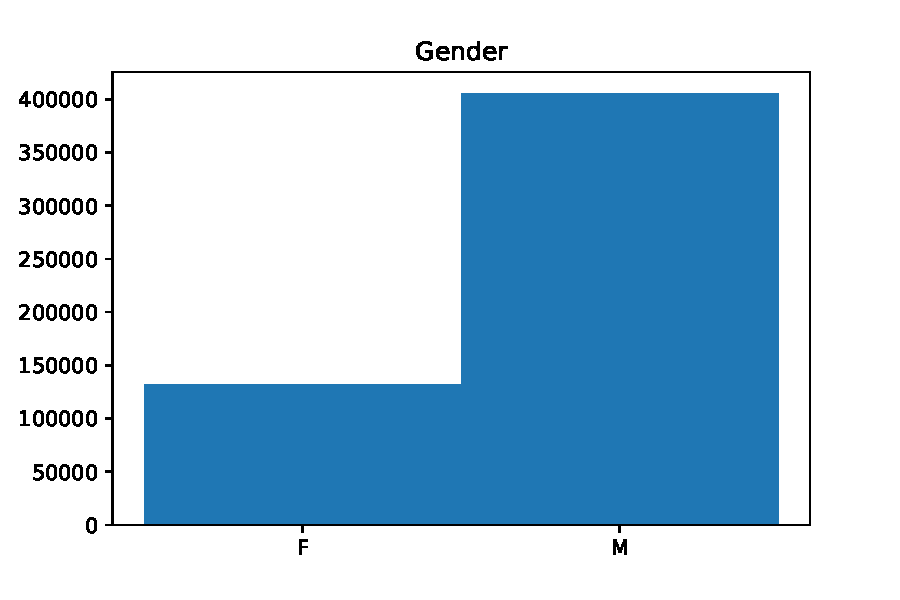
\includegraphics[width=0.49\textwidth]{plots/explore_Gender.pdf}
    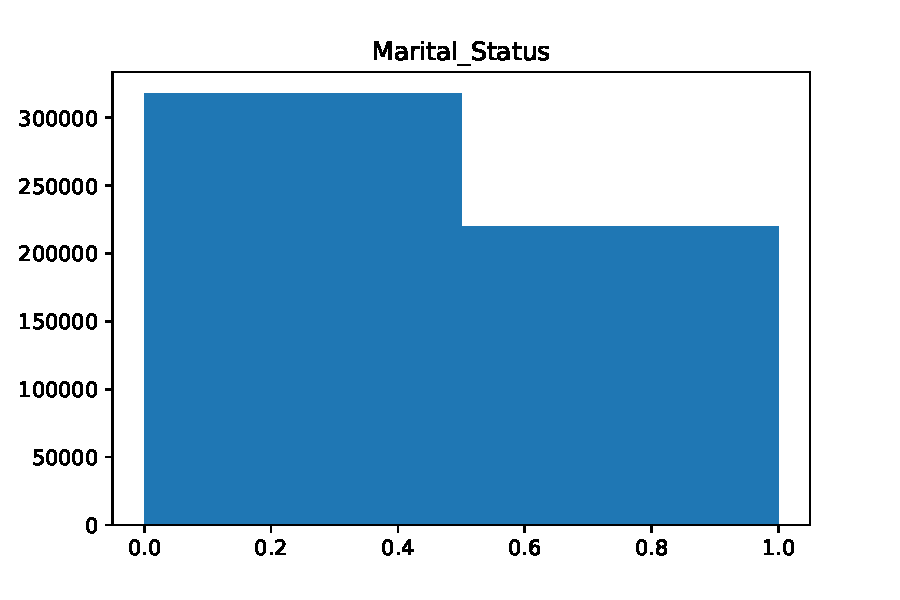
\includegraphics[width=0.49\textwidth]{plots/explore_Marital_Status.pdf}
    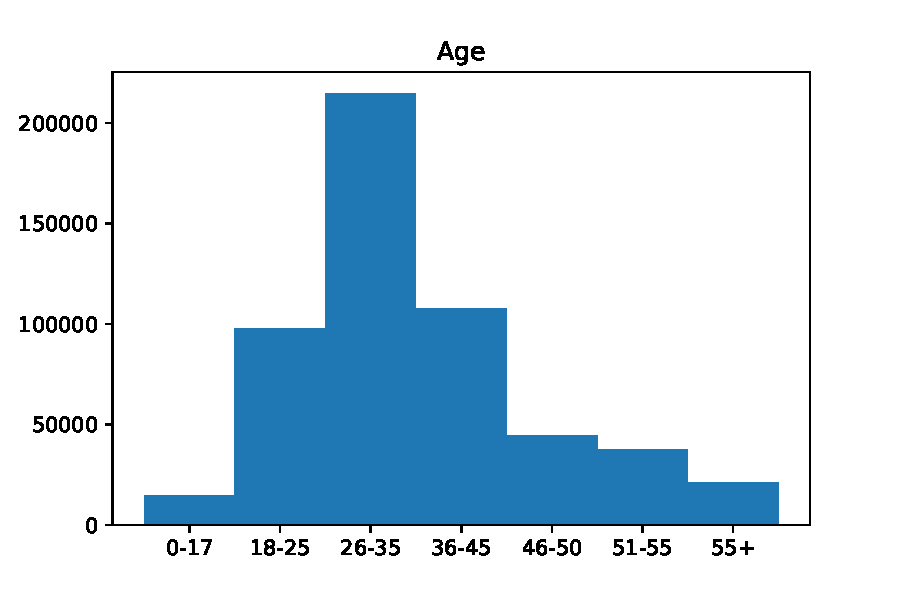
\includegraphics[width=0.49\textwidth]{plots/explore_Age.pdf}
    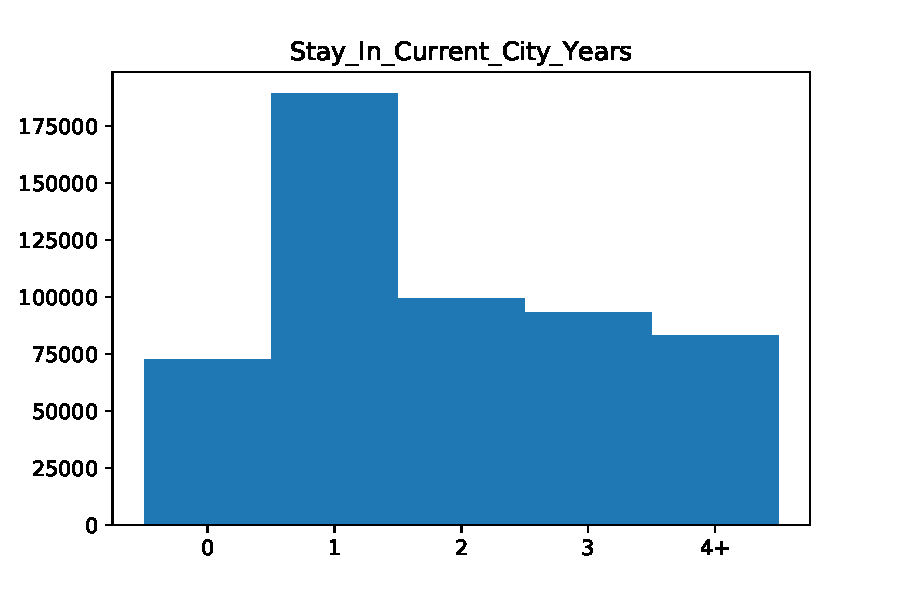
\includegraphics[width=0.49\textwidth]{plots/explore_Stay_In_Current_City_Years.pdf}
    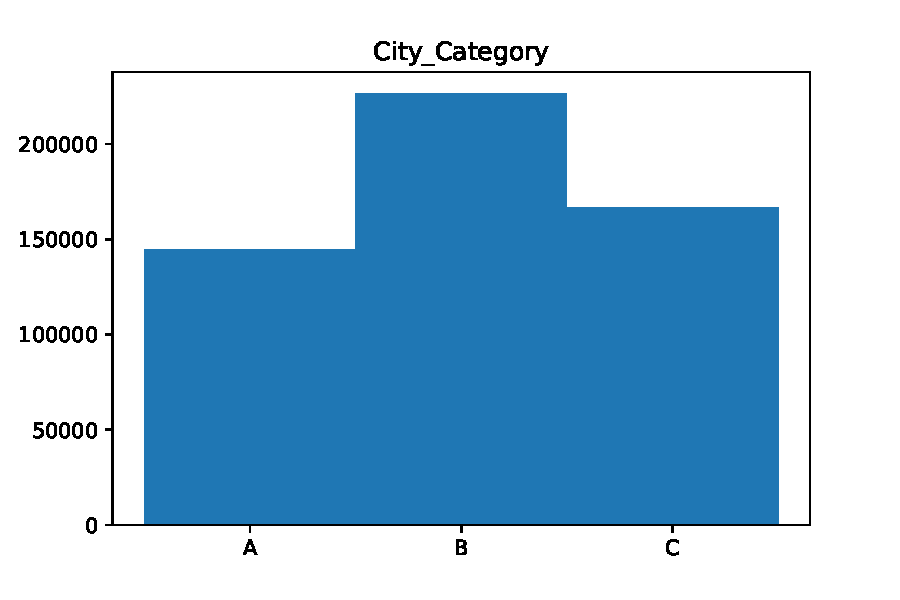
\includegraphics[width=0.49\textwidth]{plots/explore_City_Category.pdf}
    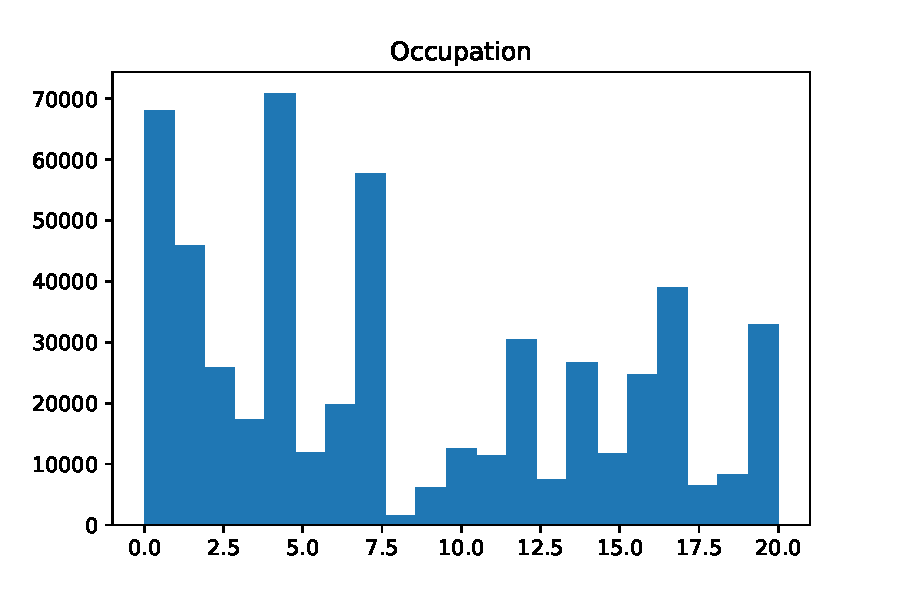
\includegraphics[width=0.49\textwidth]{plots/explore_Occupation.pdf}
    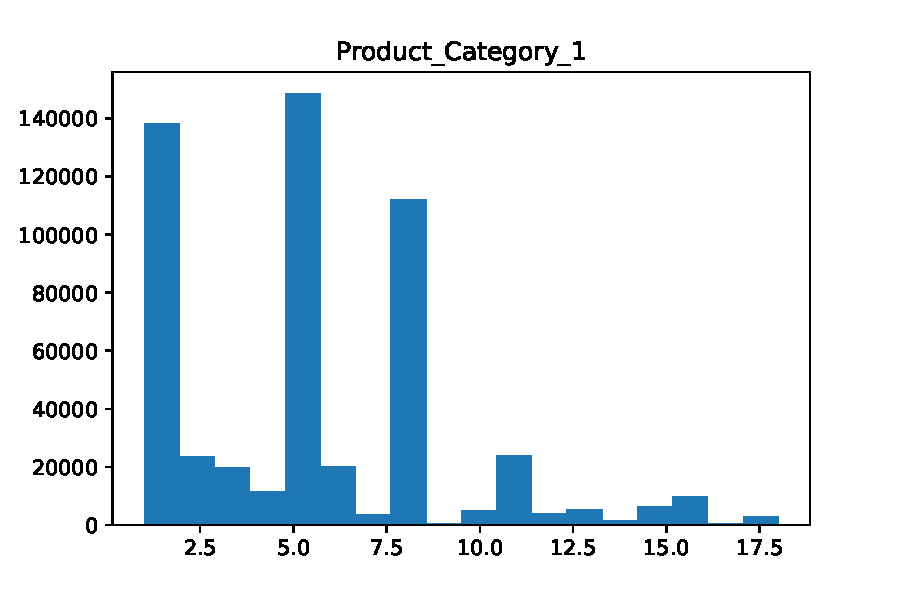
\includegraphics[width=0.49\textwidth]{plots/explore_Product_Category_1.pdf}
    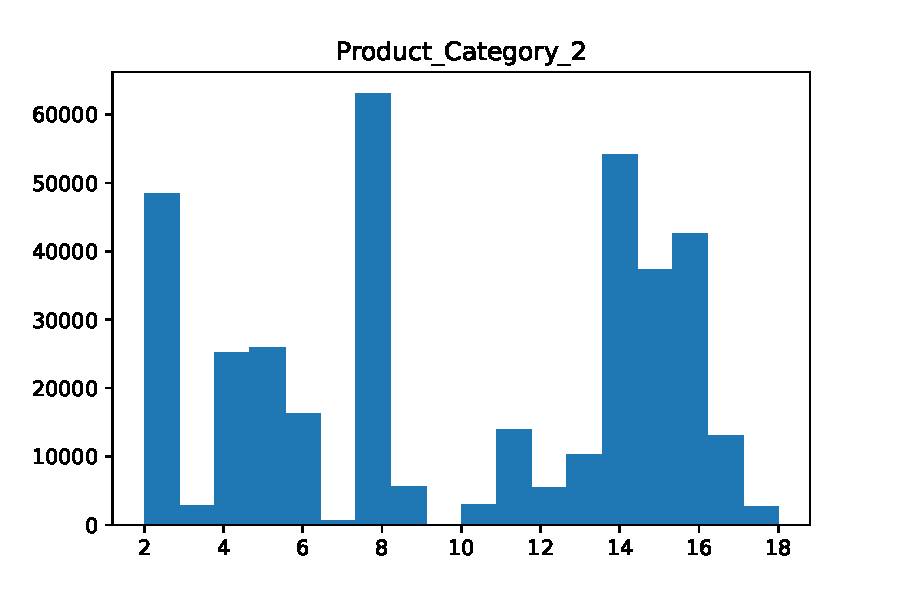
\includegraphics[width=0.49\textwidth]{plots/explore_Product_Category_2.pdf}
    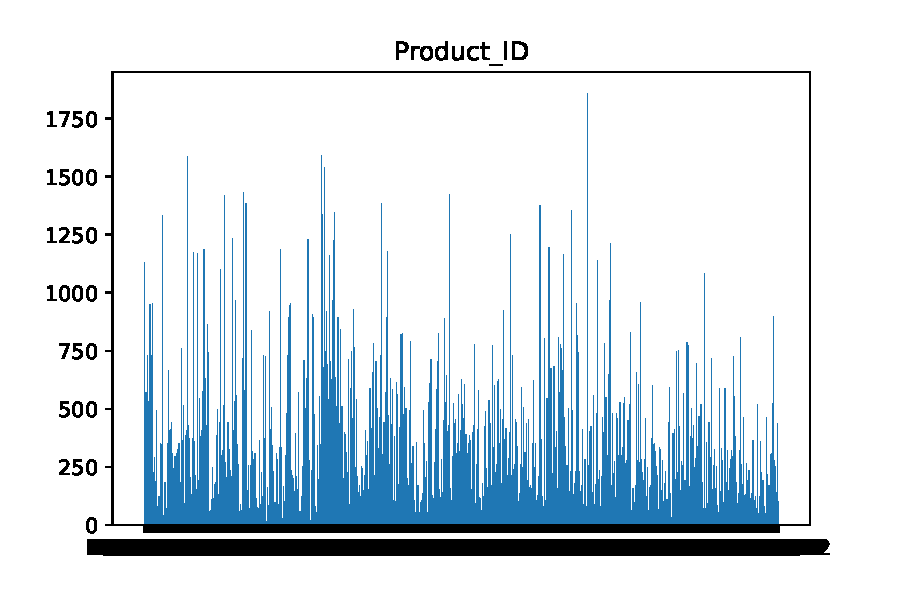
\includegraphics[width=0.49\textwidth]{plots/explore_Product_ID.pdf}
    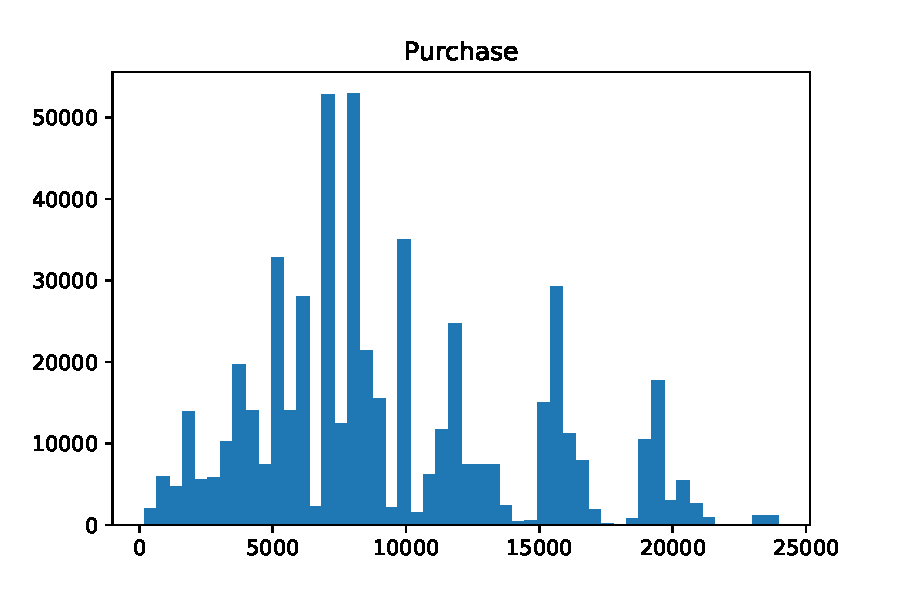
\includegraphics[width=0.49\textwidth]{plots/explore_Purchase.pdf}

  \end{center}
  \caption{Distributions of columns in the provided dataset.}
  \label{fig:exploration}
\end{figure}


\section{Data cleaning}

For easier handling the following data cleaning was performed:
\begin{itemize}
\item Product IDs,  "city category", and "Stay in current city years" were converted to integers
\item Gender was encoded as integer (Male = 1, Female = 0)
\item Age was also encoded as integer taken as the middle of the interval (could sample uniform distro between the edges instead)
\end{itemize}

\section{Best-selling and most profitable products}

The number of products sold varies dramatically (a power law, as could be expected) as does the income they generate (sum over purchase for the same product ID). The distributions are shown in Figure \ref{fig:profit}. Most frequently sold products are shown in Table \ref{tab:frequency} and those generating the most revenue are shown in Table \ref{tab:revenue}.

\begin{figure}[h]
  \begin{center}
      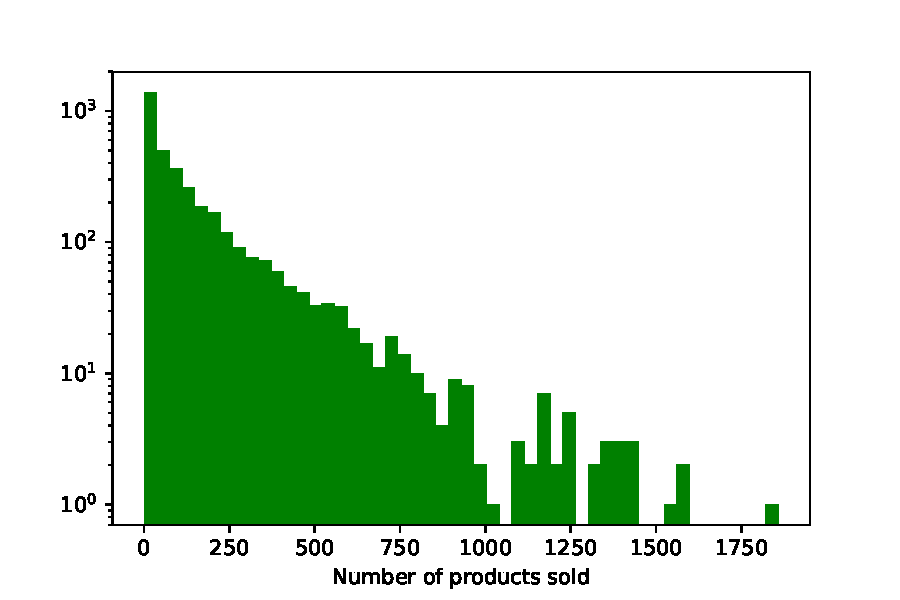
\includegraphics[width=0.49\textwidth]{plots/products_Numberofproductssold.pdf}
    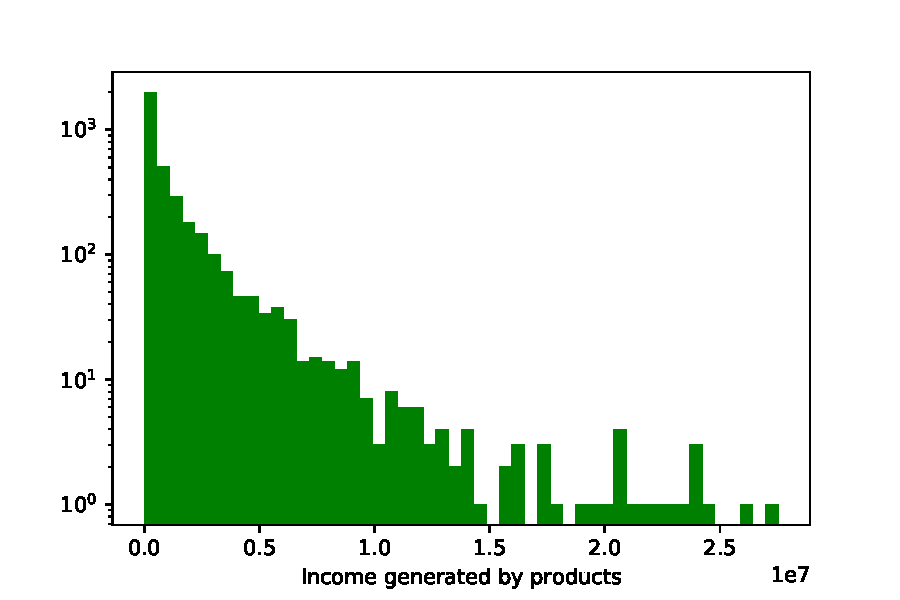
\includegraphics[width=0.49\textwidth]{plots/products_Incomegeneratedbyproducts.pdf}
  \end{center}
  \caption{Distribution of number of products sold (left) and income they generated (right). The tails of the distribution are interesting, these are the few products which are sold the most often and those which generate the most revenue.}
  \label{fig:profit}
\end{figure}

\begin{table}[h]
  \medskip
  \centering
  \begin{tabular}{l l}
    \toprule
    Product ID & Number of times sold    \\
    \midrule
    
    265242   & 1858 \\
    110742   & 1598 \\
    25442    & 1588 \\
    112142   & 1538 \\
    57642    & 1438 \\
    184942   & 1428 \\
    46742    & 1418 \\
    58042    & 1398 \\
    59442    & 1388 \\
    145042   & 1388 \\
    
    \bottomrule
  \end{tabular}
  \medskip
  \caption{Most frequently sold products.}
  \label{tab:frequency}
\end{table}


\begin{table}[h]
  \medskip
  \centering
  \begin{tabular}{l l}
    \toprule
    Product ID & Total revenue generate    \\
    \midrule
 
    25442     & 27532426\\
    110742    & 26382569\\
    255842    & 24652442\\
    184942    & 24060871\\
    59442     & 23948299\\
    112142    & 23882624\\
    110942    & 23232538\\
    237542    & 23096487\\
    57642     & 22493690\\
    10742     & 21865042\\

    \bottomrule
  \end{tabular}
  \medskip
  \caption{Products generating the most revenue.}
  \label{tab:revenue}
\end{table}


\section{Best customers}

Let's explore what demographic group buys the most products and spends the most money. See Figure \ref{fig:customers} for details. Perhaps surprisingly the differences between demographic groups are quite small, but nevertheless there are a few patterns:

\begin{itemize}
\item Older customers spend more dollar, probably because more dollar is available.
\item There are differences between city categories of the same size.
\item Males spend more.
\item There are differences between occupations.
\end{itemize}

All of these differences are likely correlated with how much money people make. For some it is obvious (age, gender pay gap), while occupations and city category can only be speculated.

\begin{figure}[h]
  \begin{center}
    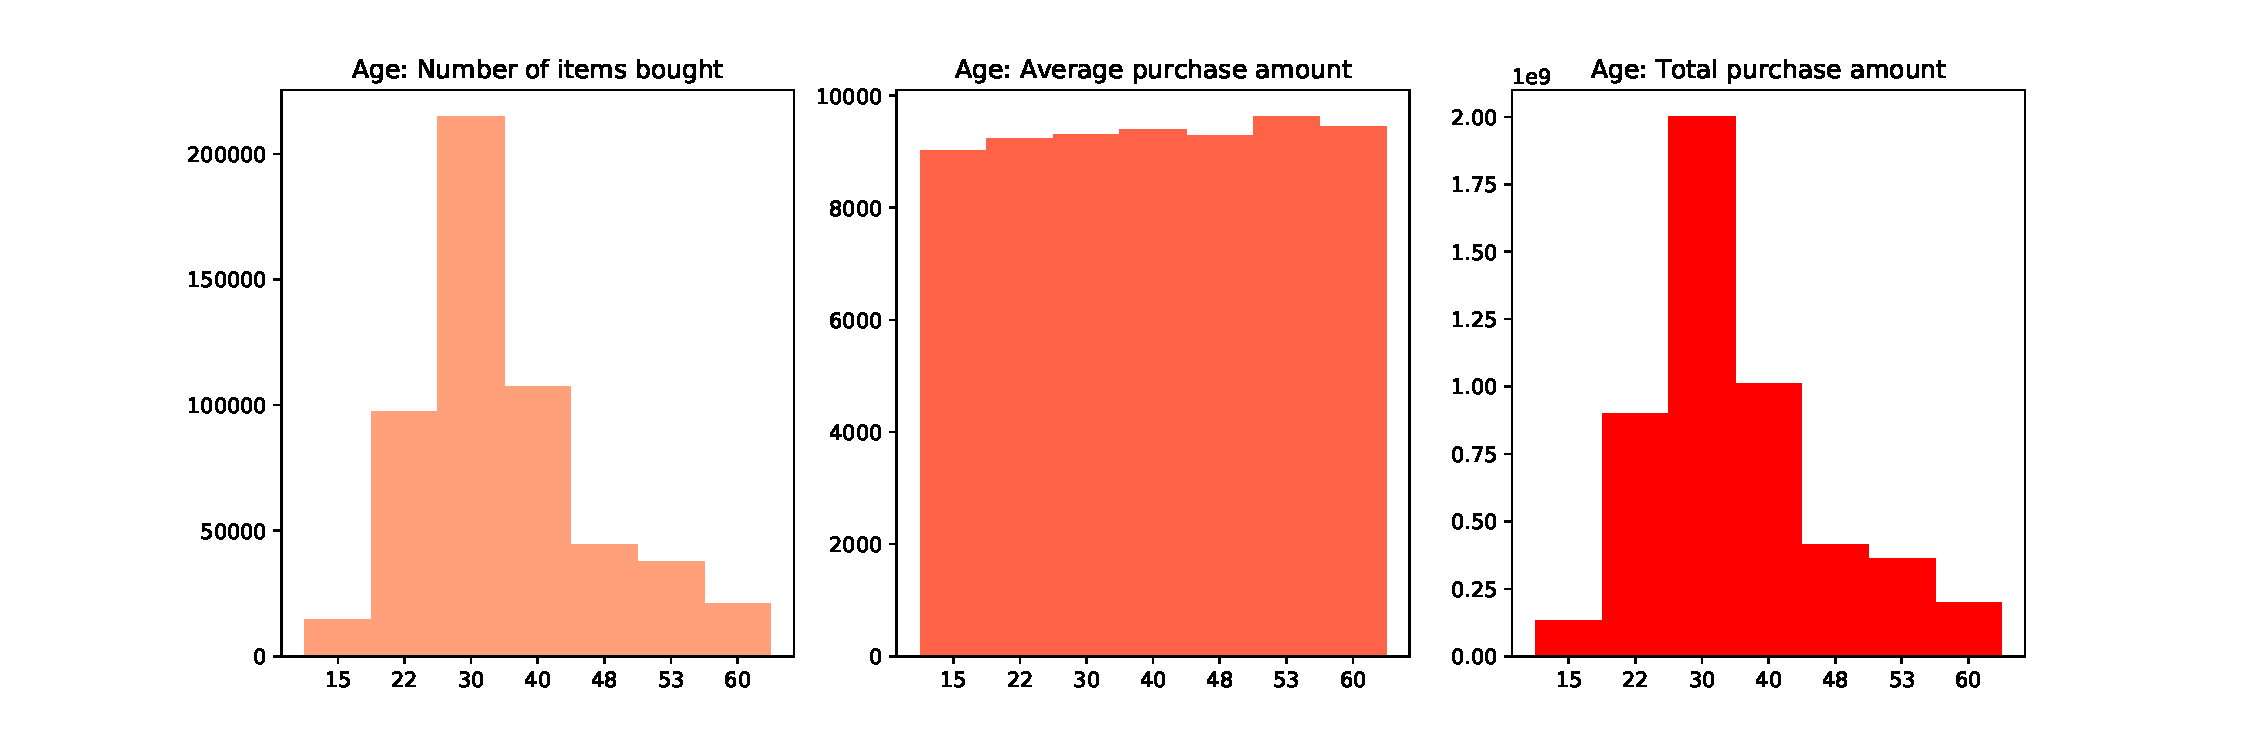
\includegraphics[width=0.99\textwidth]{plots/customers_Age.pdf}
    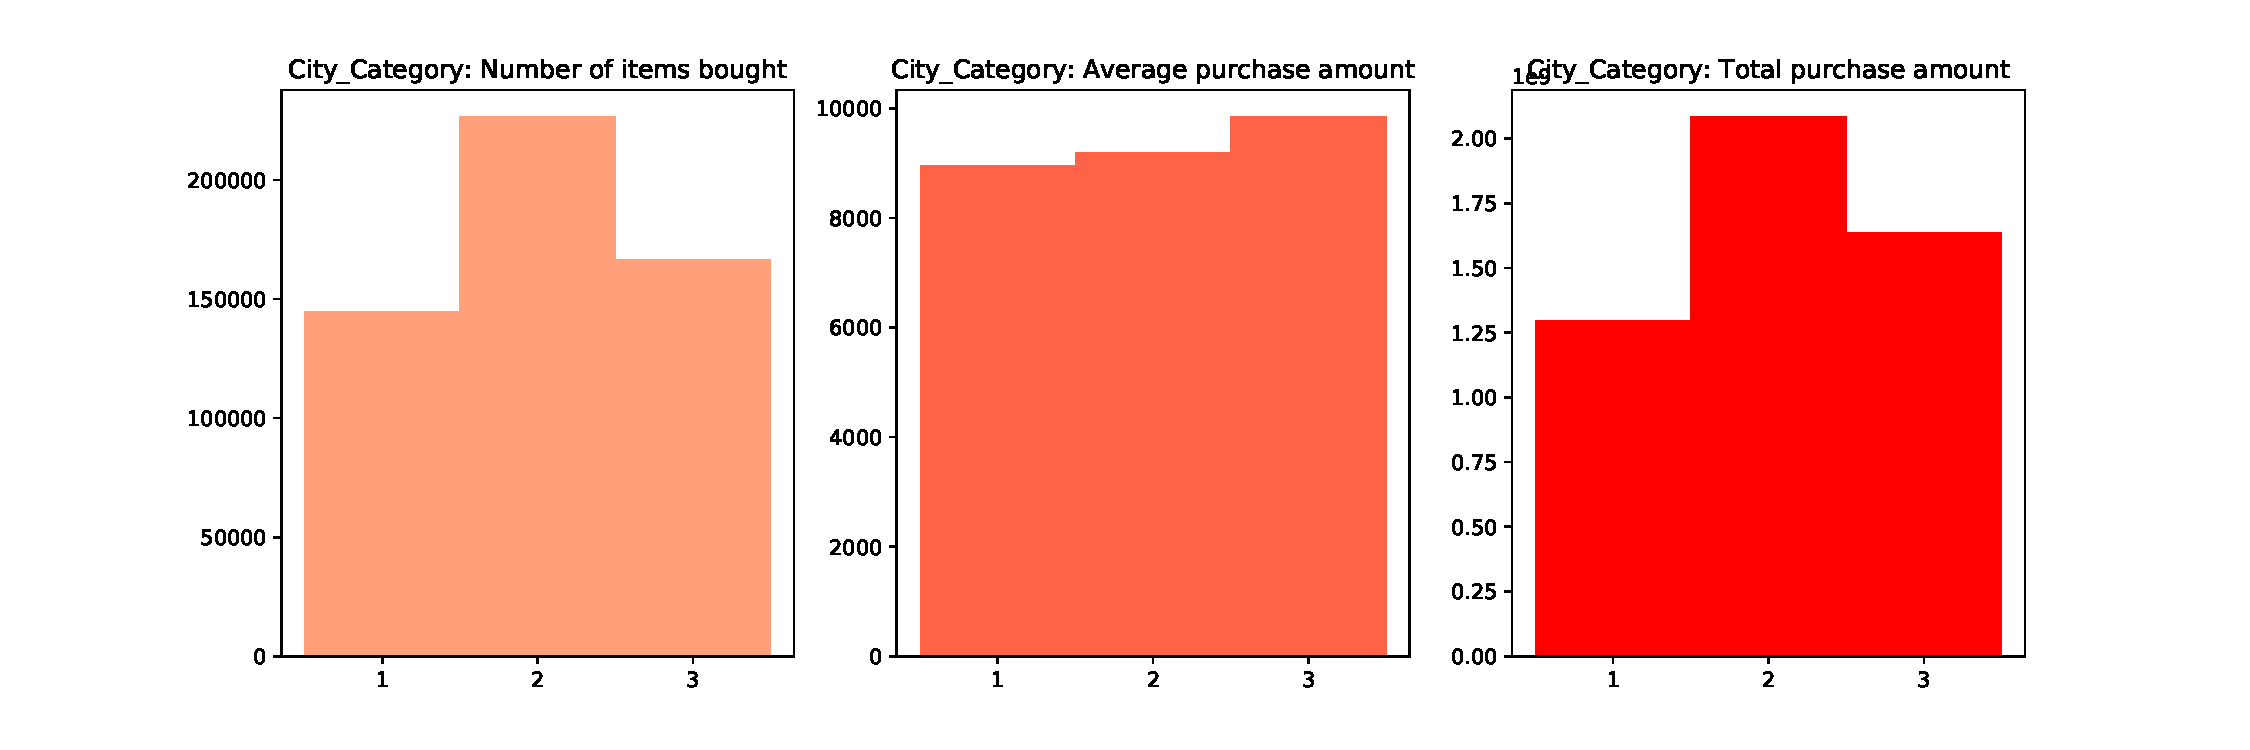
\includegraphics[width=0.99\textwidth]{plots/customers_City_Category.pdf}
    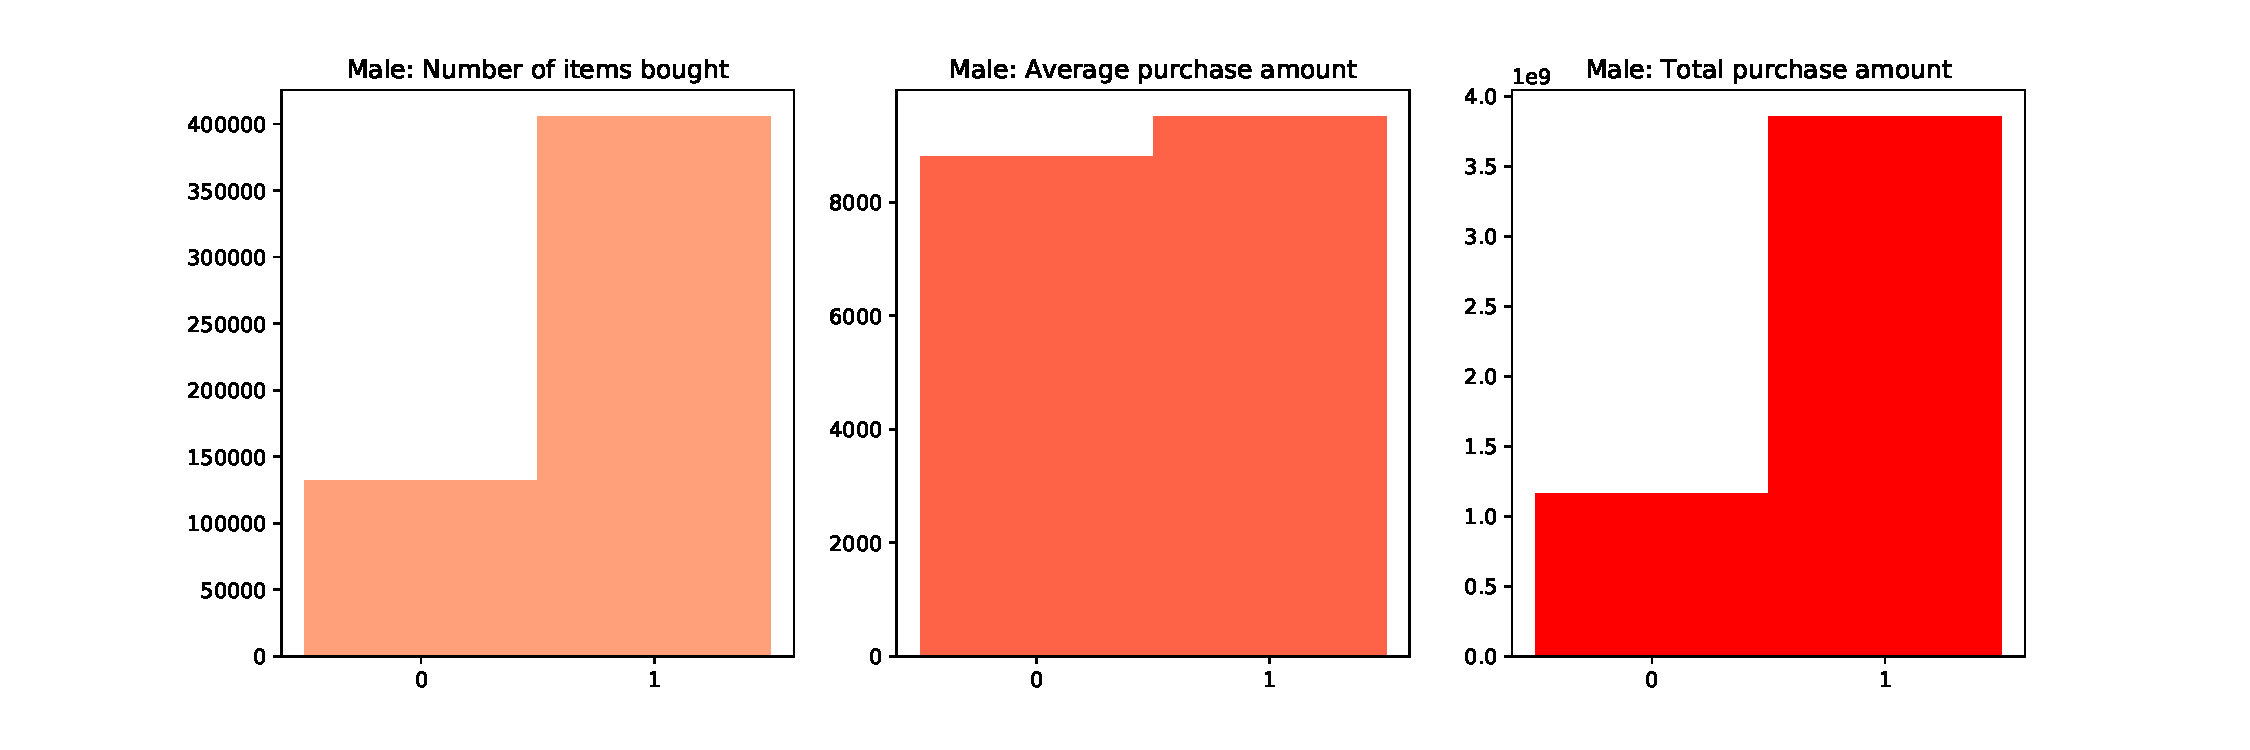
\includegraphics[width=0.99\textwidth]{plots/customers_Male.pdf}
    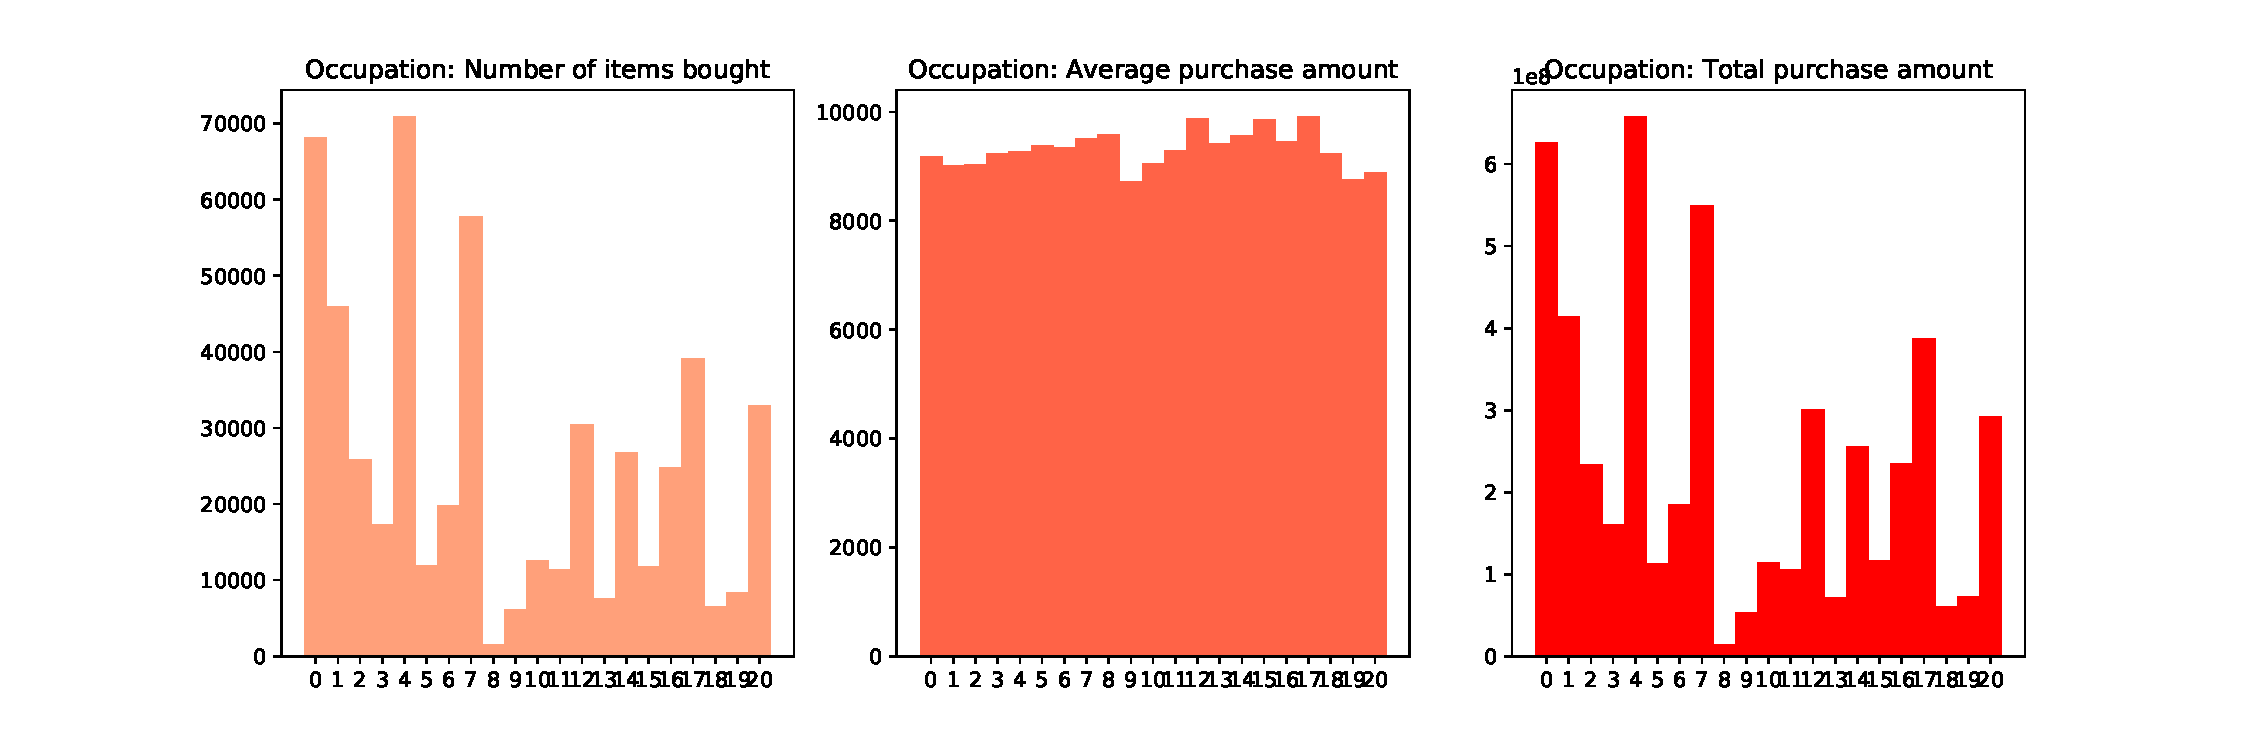
\includegraphics[width=0.99\textwidth]{plots/customers_Occupation.pdf}

  \end{center}
  \caption{Customer analysis. Left plot shows the number of items bought per demographic group, the middle one represents the average purchase amount and the right represents total purchase amount.}
  \label{fig:customers}
\end{figure}


\section{The simplest of recommender systems}

I've written some hacky code to build a network of which products are related, represented by a matrix. Essentially, when items are bought by the same customer, the weight of the edge increases by 1. In the end, the matrix is normalised by the frequency of the items to avoid always recommending the same item. I'm sure there are technical names for this but I've never studied this...

Anyway, this network is then read by another hacky function which takes a product and returns N products with the highest score in the network.

This could be used for targeted ads for customers, especially if contact information is available. If there is an online shop available for this retailer, suggestions could pop up there too.

\section{Predicting how much customers will spend}

Now let's get fancy and predict Purchase column from (most of) other info available. I've used the GradientBoostingRegressor from sklearn and ran out of time to compare it to xgboost.

\paragraph{Training and performance} Data was split in training and test sets. I've used repeated kfold CV on the training data to select the best hyperparameters for the model. The model was then trained on the entire training set and its performance and an error on that performance were evaluated by bootstrapping the test set. The average absolute deviation in the prediction was found to be 2118.3 +/- 3.9.

Better performance could be achieved by feature engineering (say add average purchase for product id or product category as a column) and by optimising over a larger set of hyperparameters (just done the learning rate and maximum depth of individual learners). XGboost would probably be even better. Deep nets probably too though but probably only after quite extensive tuning and preprocessing and I felt it wasn't really worth it in this case.


\paragraph{Usage of the model}

Based on the previous results one could design a marketing strategy to target the customers in the demographic groups which spend a lot but are currently not well represented - put more ads on TV for example, old people watch that. After having a realistic estimate of how successful the campaign is (i.e. how many more people will show up in the store on the day) one can use this model to see how this impacts the sales, and whether the advertising campaign was worth it.

\paragraph{Possible extensions}

One could build a probabilistic model to predict what people will buy, and again fold that in with the predicted demographics that would visit on the day to calculate what to stock up on. 

\section{Future}

Do collect time information on when the products were sold (year and hour) to be able to track demand over time, as well as find out whether the item was sold out on the day.

%%%%%%%%%%%%%%%%%%%%%%
% REFERENCES
%%%%%%%%%%%%%%%%%%%%%%

\small
\bigskip
\bigskip
\bibliographystyle{unsrt}
\bibliography{mwe}
\addcontentsline{toc}{section}{References}



\end{document}
